\newpage
\section{Sterowanie obiektu}
\subsection{Klasyczny DMC}
Na początek zdecydowano się przetestować klasyczny algorytm DMC. W tym celu zebrano odpowiedź skokową w punkcie pracy. Została ona przedstawiona na rysunku \ref{fig:normalDMCs}.
\begin{figure}[!h]
	\centering 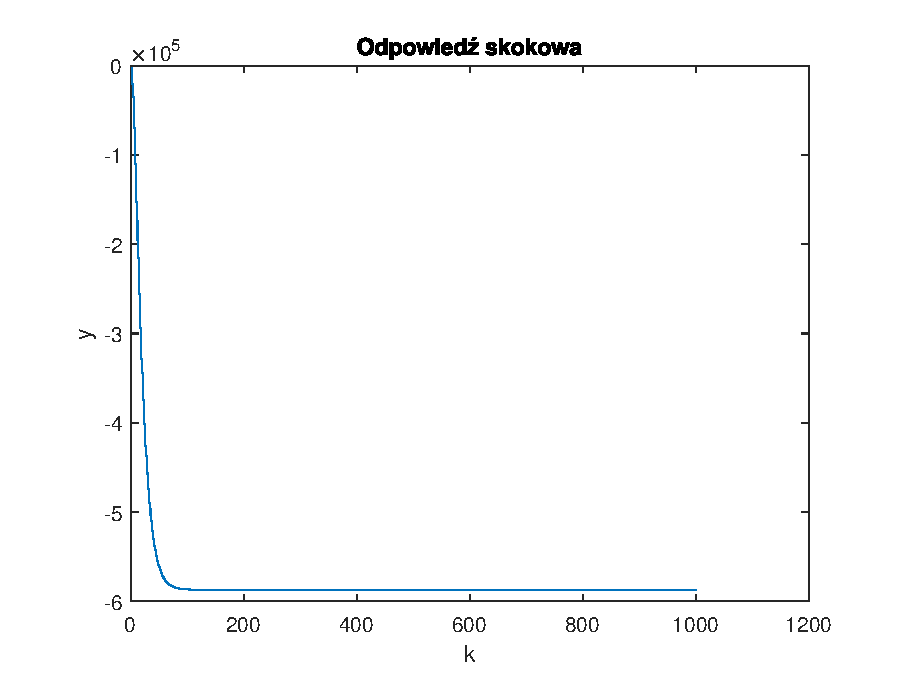
\includegraphics[width=0.8\linewidth]{normalDMCs.eps}
	\caption{Odpowiedź skokowa dla klasycznego algorytmu DMC}
	\label{fig:normalDMCs}
\end{figure}
Zaimplementowano algorytm DMC w wersji analitycznej. Przyjęto parametry regulatora $D =200$, $N= 200$, $N_U = 200$, $\lambda=1e+8$. Zostały one dobrane eksperymentalnie. Przebieg dla przykładowej trajektorii wartości zadanej został przedstawiony na rysunku \ref{fig:normalDMC}.
\begin{figure}[!h]
	\centering 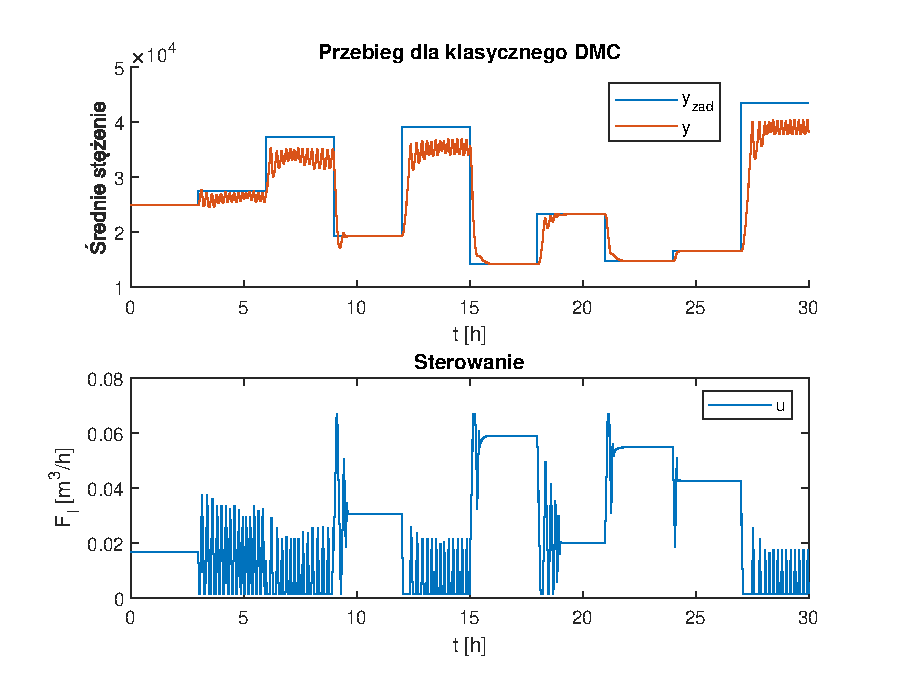
\includegraphics[width=0.8\linewidth]{normalDMC.eps}
	\caption{Przebieg dla klasycznego algorytmu DMC}
	\label{fig:normalDMC}
\end{figure}

Jak widać regulator nie radzi sobie dobrze, występują duże oscylacje, oraz uchyby ustalone. Warto też zauważyć że parametr $\lambda$ jest bardzo duży. Błąd dla tego przebiegu wyniósł 5,5095e+10. Eksperyment ten pokazuje że w przypadku badanego reaktora istnieje potrzeba zastosowania algorytmu regulacji opartego na modelu nieliniowym.

\subsection{DMC-SL}
Do zaprojektowania regulatora DMC-SL w wersji analitycznej wykorzystano odpowiedź skokową modelu dynamicznego z poprzedniego punktu. Została ona przedstawiona na rysunku \ref{fig:DMC-SLs}.
\begin{figure}[H]
	\centering 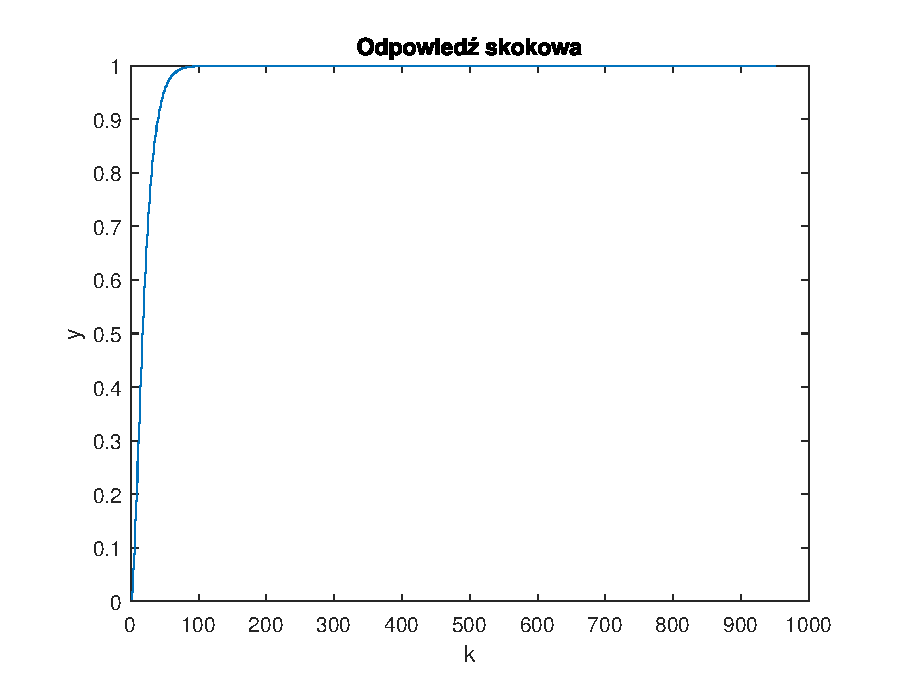
\includegraphics[width=0.8\linewidth]{DMC-SLs.eps}
	\caption{Odpowiedź skokowa dla algorytmu DMC-SL}
	\label{fig:DMC-SLs}
\end{figure}
W każdej iteracji jest ona przemnażana przez współczynnik $\alpha(k)$, co daje odpowiedź skokową w danej chwili. Wszystkie parametry regulatora są takie same jak w poprzednim podpunkcie. Przebieg dla tego regulatora został przedstawiony na rysunku \ref{fig:DMC-SL}.
\begin{figure}[H]
	\centering 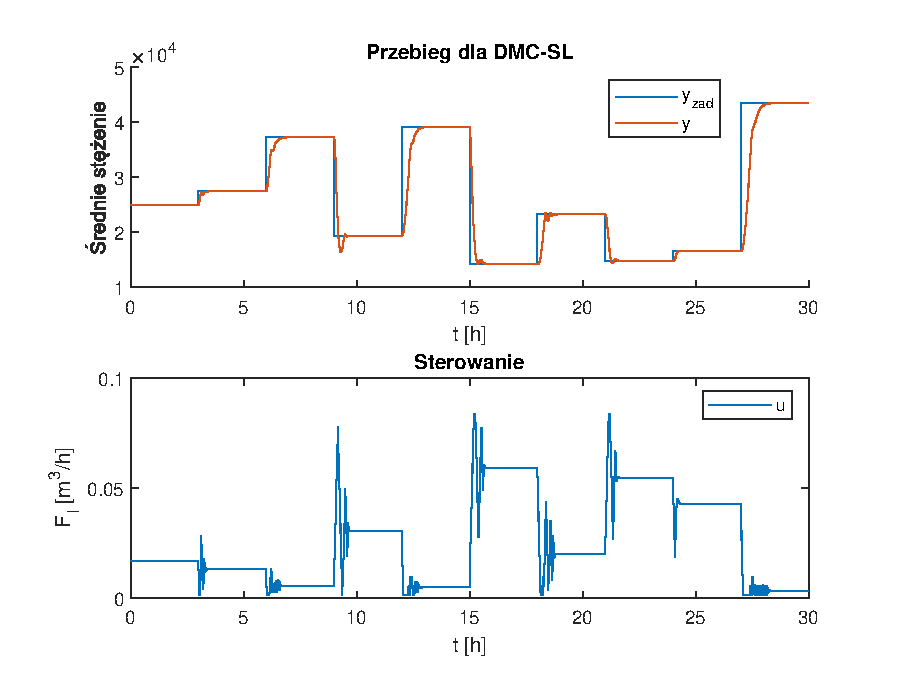
\includegraphics[width=0.8\linewidth]{DMC-SL.eps}
	\caption{Przebieg dla algorytmu DMC-SL}
	\label{fig:DMC-SL}
\end{figure}
Jak widać przebieg jest znacznie bardziej stabilny, nie występują też żadne uchyby ustalone. Błąd też uległ poprawie, był równy 4.0812e+10. Wykorzystanie zaprojektowanego modelu daje znaczne korzyści w przypadku obiektu nieliniowego z którym mamy tutaj do czynienia. Można dostroić parametry tego regulatora. Na przykład warto rozważyć zmniejszenie współczynnika $\lambda$, co powinno zwiększyć szybkość regulacji, kosztem bardziej gwałtownego przebiegu sterowania i szansy na pojawienie się oscylacji.